\documentclass{article}

\usepackage{graphicx}
\usepackage[a4paper, total={6in, 9in}]{geometry}
\usepackage{amsmath}
\usepackage{amsfonts}
\usepackage{mathtools}
\usepackage{scalerel,amssymb}
\usepackage{mathrsfs}
\usepackage{fancyhdr}
\usepackage[version=4]{mhchem}

\title{L'énergie des étoiles : la fusion nucléaire}
\author{Thomas Calvao}
\date{Avril 2025}
\begin{document}

\pagestyle{fancy}
\fancyfoot[R]{Calvao - 2024-2025}
\fancyfoot[L]{$\mathbb{MPSI}$}
\setlength{\headheight}{14pt}
\addtolength{\topmargin}{-2pt}

\maketitle
\tableofcontents
\vfill

Lors de ce TIPe, nous allons étudier la puissance des réactions de fusion de ce modèle. Dans un premier temps, nous allons tracé la courbe de la puissance des réactions en fonction de la température et de la quantité de matière initial. Ensuite, nous allons appliqué ce modèle au projet ITER (quantité de matière, température). Nous allons enfin comparé la puissance de ces réactions dans ce cas particulier, en prenant en compte le rendement du réacteur ainsi que la puissance nécessaire pour le fonctionnement du réacteur.
\newpage

\noindent Quelles sont les conditions nécessaires au maintien continu d’une réaction de fusion nucléaire dans
un environnement confiné ?

\section{Présentation du code}

\subsection{Esthétique}

\begin{figure}[h]
    \centering
    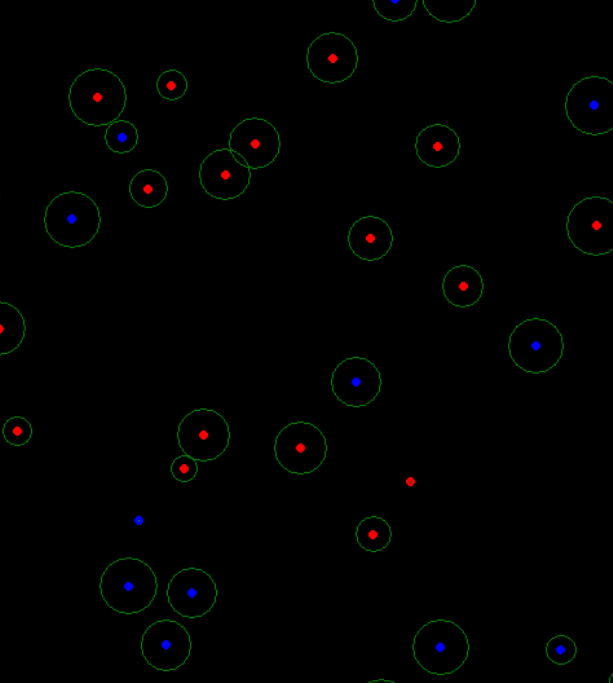
\includegraphics[width=0.5\linewidth]{Images/Image Code.png}
    \caption{Capture d'écran de la simulation (zoomé)}
    \label{fig:code}
\end{figure}
Voici un schéma de ce à quoi doit ressembler le code. \\
Légende :
\begin{itemize}
    \item Les points rouge représentent les atomes de deutérium
    \item Les points bleu représentent les atomes de tritium
    \item Les cercles vert représentent les sections efficaces de la réaction D-T
    \item Les bords noirs sont des bords sans fin : lorsque un atome traverse un bord, il réapparaît de l'autre coté. Le volume étudié est un tore.
\end{itemize}

\section{Principe physique}

\subsection{Densité}

\label{densité}
Pour la densité, on se base sur les données du réacteur ITER. On prend donc une quantité de 1 gramme de réactif pour un volume de 830 m$^3$. Donc $\boxed{N=2,4\times10^{23}\text{ particules}}$.

\subsection{Vitesse initial}

\label{maxwell}
La vitesse initial de chaque particule est calculé selon une distribution Maxwellienne.
    
\begin{figure}[ht]
    \centering
    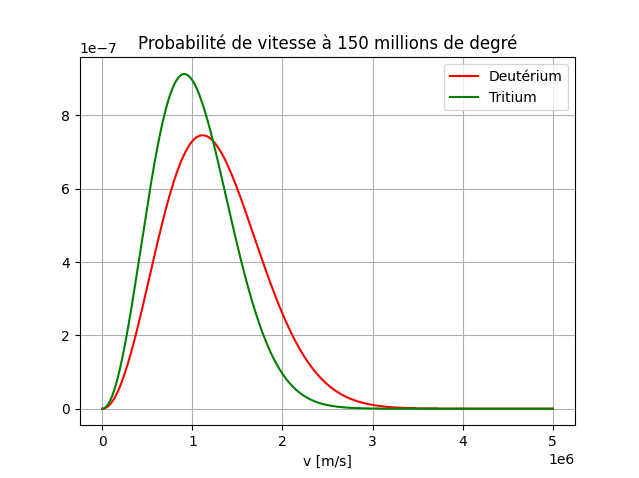
\includegraphics[width=0.5\linewidth]{Images/Probabilité de vitesse.png}
    \caption{Distribution de la norme de la vitesse du deutérium à 150 millions de degré}
    \label{fig:maxwell}
\end{figure}
Cette courbe est celle des molécule d'oxygène. On va donc tracer cette courbe pour les atomes de deutérium et de tritium pour les températures correspondantes et pour une quantité de matière égale à $\frac{n}{2}$ à l'aide de l'équation suivante :
\[ \boxed{f(v) = \sqrt{\frac{2}{\pi}}\left(\frac{m}{k_BT}\right)^\frac{3}{2}v^2\mathrm{e}^{-\frac{mv^2}{2k_BT}}} \]
avec $v$ la vitesse, $m$ la masse de chacune des particules, $T$ la température et $k_B$ la constante de Boltzmann.

\subsection{Section efficace}

\label{cross section}
La section efficace d'une réaction est une aire sphérique autour de l'atome. Dans le cadre de la fusion nucléaire, si la section efficace de deux atomes se croisent, la probabilité de fusion vaut 1. Cette valeur s'explique avec l'effet tunnel. \\
La section efficace de la réaction de Deutérium-Tritium est donnée par le graphique suivant :
\begin{figure}[ht]
    \centering
    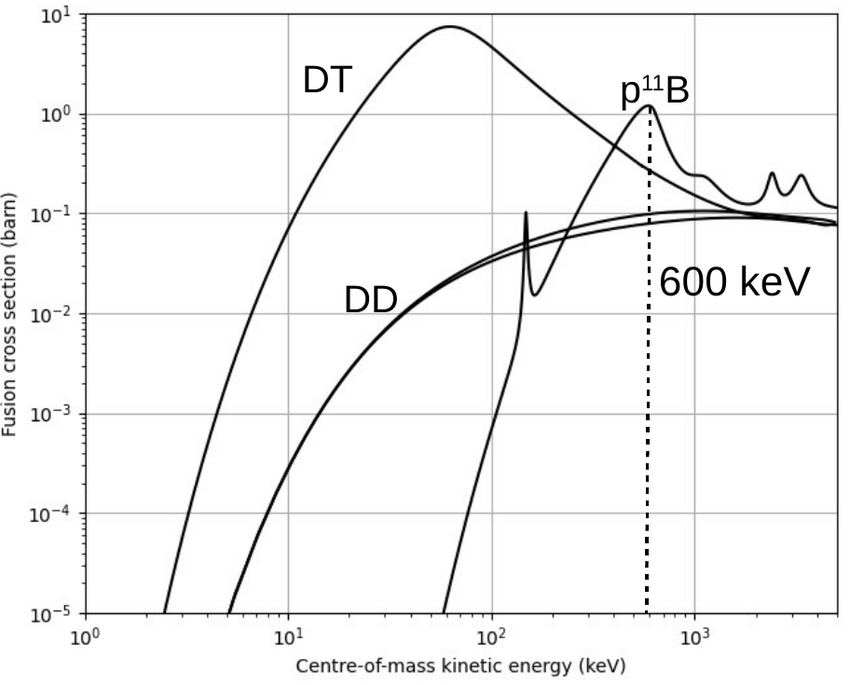
\includegraphics[width=0.5\linewidth]{Images/Fusion-cross-sections-of-Deuterium-Tritium-DT-Deuterium-Deuterium-DD-and.png}
    \caption{Section efficace d'une particule en fonction de son énergie}
    \label{fig:cross_section}
\end{figure}
Pour la modélisation, nous allons devoir approximé linéairement à l'aide de python la section efficace de la réaction de deutérium-tritium. \\
Étant donné que la vitesse des particules n'est pas constante dans le plasma, leur température ne l'est pas non plus. Il faut donc recalculer la section efficace de chaque particule à chaque instant de la simulation. \\
Nous approximerons la section efficace grâce à cette image :
\begin{figure}[ht]
    \centering
    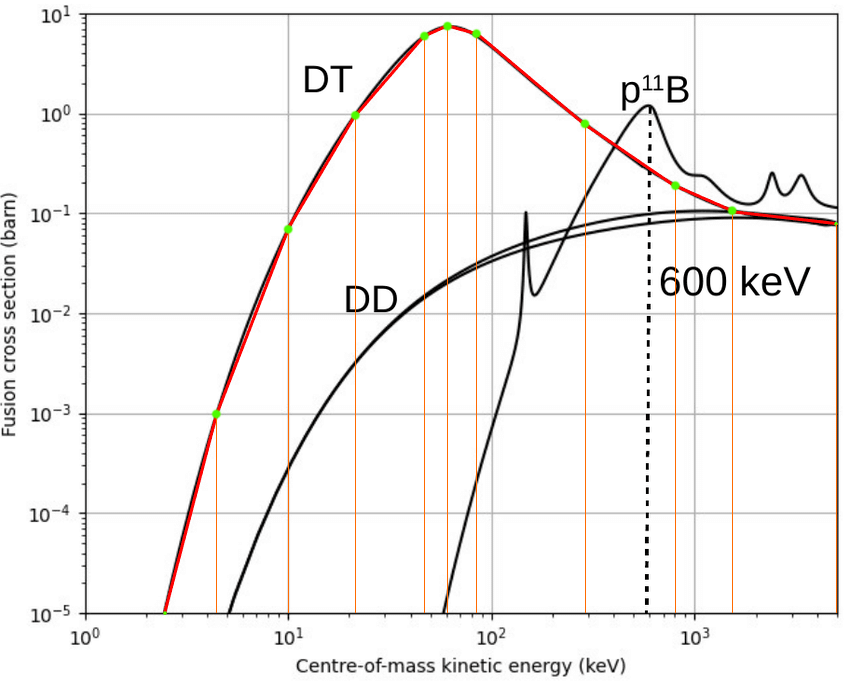
\includegraphics[width=0.5\linewidth]{Images/Fusion-cross-sections-of-Deuterium-Tritium-DT-Deuterium-Deuterium-DD-and(mod).png}
    \caption{Approximation linéaire}
    \label{fig:enter-label}
\end{figure}

\subsection{Énergie}

\label{energie}
L'énergie des réactions de fusion est calculé à partir de la relation $E=mc^2$. La réaction étudiée est la suivante :
\[ \ce{^{2}_{1}H} + \ce{^{3}_{1}H} \longrightarrow \ce{^{4}_{2}He} + \ce{^{1}_{0}n} \]
Calculons les masses des différents membres de l'équation : \\
\underline{Membre de gauche :} \[ (2 - 0.000994)\text{ m}_\text{proton} + (3 - 0.006284)\text{ m}_\text{proton} = 4.992722\text{ m}_\text{proton} \]
\underline{Membre de droite :} \[ (4 - 0.027404)\text{ m}_\text{proton} + (1 + 0.001378)\text{ m}_\text{proton} = 4.973974\text{ m}_\text{proton} \]
On observe donc une différence de masse $\Delta$m entre le membre de gauche et le membre de droite. C'est cette différence de masse qui est transformé en énergie. On a donc
\begin{align*}
    \Delta\text{m} &= 4.992722\text{ m}_\text{proton} - 4.973974\text{ m}_\text{proton} \\
        &= 0.018747\text{ m}_\text{proton} \\
        &\boxed{= 3.135790\times10^{-29}\text{ kg}}
\end{align*}
\begin{flalign*}
    \text{D'où}\quad E &= \Delta\text{m}c^2 &\\
    &= 3.135790\times10^{-29}\times\left(2.9979\times10^{8}\right)^2 &\\
    &= 2.8182\times10^{-12}\text{ J} &\\
    &\boxed{= 17.59\text{ MeV}}
\end{flalign*}
On obtient donc que chaque réaction de fusion produit une énergie de 17,59 MeV.

\subsection{Force}

Le poid de chaque particule est négligé. La seul force s'appliquant sur chaque particule est donc :
\[ \vec{F_e} = \frac{q^2}{4\pi\varepsilon_0}\times\frac{1}{r^2}\vec{u_r} \]

\subsection{Puissance}

\label{puissance}
La puissance des réactions sera calculé comme la dérivée de l'énergie libéré par les réactions de fusion.

\subsection{Volume et dimension}

\label{Volume et dimension}
La taille de la zone est calculé automatiquement. Pour un cylindre, on a que
\[ V = 2\pi^2Rr^2 \]
De plus, on pose un ration entre $2\pi(R-r)$ et $2\pi r$. En effet :
\[ \frac{R-r}{r} = q =\frac{16}{9} \]
On en déduit un système de deux équations qui nous permet d'obtenir les expressions suivantes :
\begin{align*}
    r &= \sqrt[3]{\frac{V}{2\pi^2(q+1)}} \\
    R &= (q+1)\times r
\end{align*}
On peut alors calculer les dimensions de la zone simulé en fixant le volume. \\
Enfin, on dispose d'une zone de 1600 par 900 pixel. On en déduit donc le nombre de mètre par pixel noté $m_p$ :
\[ m_p = \frac{2\pi(R-r)}{1600} = \frac{2\pi r}{900} \]
En prenant les dimensions d'ITER, on a un volume de 830 m$^3$. Cependant, pour $V = 830\text{ m}^3$, $N=2,4\times10^{23}$ ce qui n'est pas simulable. En prenant $N=1000$, on obtient $V = 3,4\times10^{-18}\text{ m}^3$. Enfin, on obtient :
\begin{align*}
    N &= 1000 \\
    V &= 3,4\times10^{-18}\text{ m}^3 \\
    r &= 3,9\times10^{-7}\text{ m} \\
    R &= 1,0\times10^{-6}\text{ m}
\end{align*}
D'où
\[ m_p \approx 5\times10^{-10}\text{ m/pixel} \]
On obtient alors un modèle conservant la densité du réacteur ITER tout en aillant des dimensions simulablent dans des temps convenables et en gardant une fluidité de la simulation.

\end{document}
